\section{Zbiór Glass}
\subsection{Algorytm Adaboost}

\begin{tabular}{llrrrrrrrr}
\hline
          & \{\} & \multicolumn{8}{l}{Miara F1} \\
          & Liczba foldów &        2 &      3 &      4 &      5 &      6 &      7 &      8 &      9 \\
Parametr & Wartość parametru &          &        &        &        &        &        &        &        \\
\hline
algorithm & SAMME &    0.557 &  0.647 &  0.667 &  0.624 &  0.645 &  0.630 &  0.687 &  0.693 \\
          & SAMME.R &    0.586 &  0.611 &  0.662 &  0.616 &  0.685 &  0.713 &  0.686 &  0.689 \\
\hline
\end{tabular}

\begin{figure}[H]
    \center
    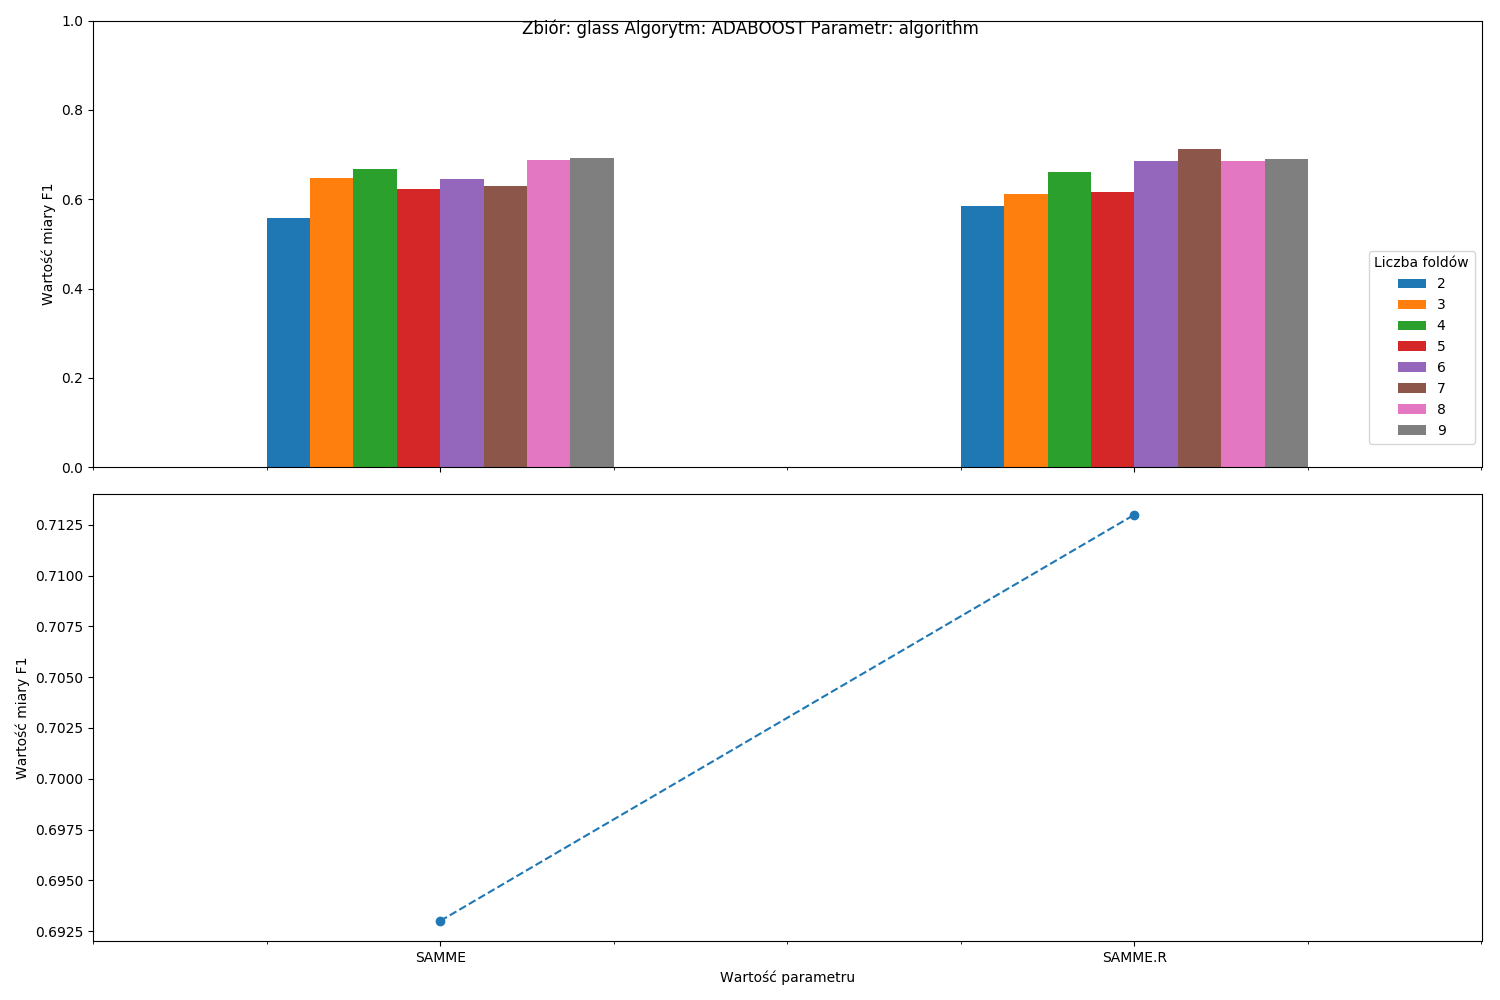
\includegraphics[width=\textwidth]{resources/plots/glass_adaboost_algorithm.png}
    \caption{Wykres wartości miary F1 dla zbioru "Glass" algorytmu "Adaboost" przy ustalonym parametrze "algorithm".}   
\end{figure}

\pagebreak
                    
\begin{tabular}{llrrrrrrrr}
\hline
              & \{\} & \multicolumn{8}{l}{Miara F1} \\
              & Liczba foldów &        2 &      3 &      4 &      5 &      6 &      7 &      8 &      9 \\
Parametr & Wartość parametru &          &        &        &        &        &        &        &        \\
\hline
learning\_rate & 0.0001 &    0.440 &  0.585 &  0.661 &  0.602 &  0.600 &  0.696 &  0.679 &  0.661 \\
              & 0.001 &    0.548 &  0.565 &  0.671 &  0.629 &  0.641 &  0.661 &  0.662 &  0.644 \\
              & 0.01 &    0.513 &  0.550 &  0.623 &  0.645 &  0.653 &  0.689 &  0.719 &  0.635 \\
              & 0.1 &    0.579 &  0.568 &  0.636 &  0.655 &  0.578 &  0.668 &  0.650 &  0.699 \\
\hline
\end{tabular}

\begin{figure}[H]
    \center
    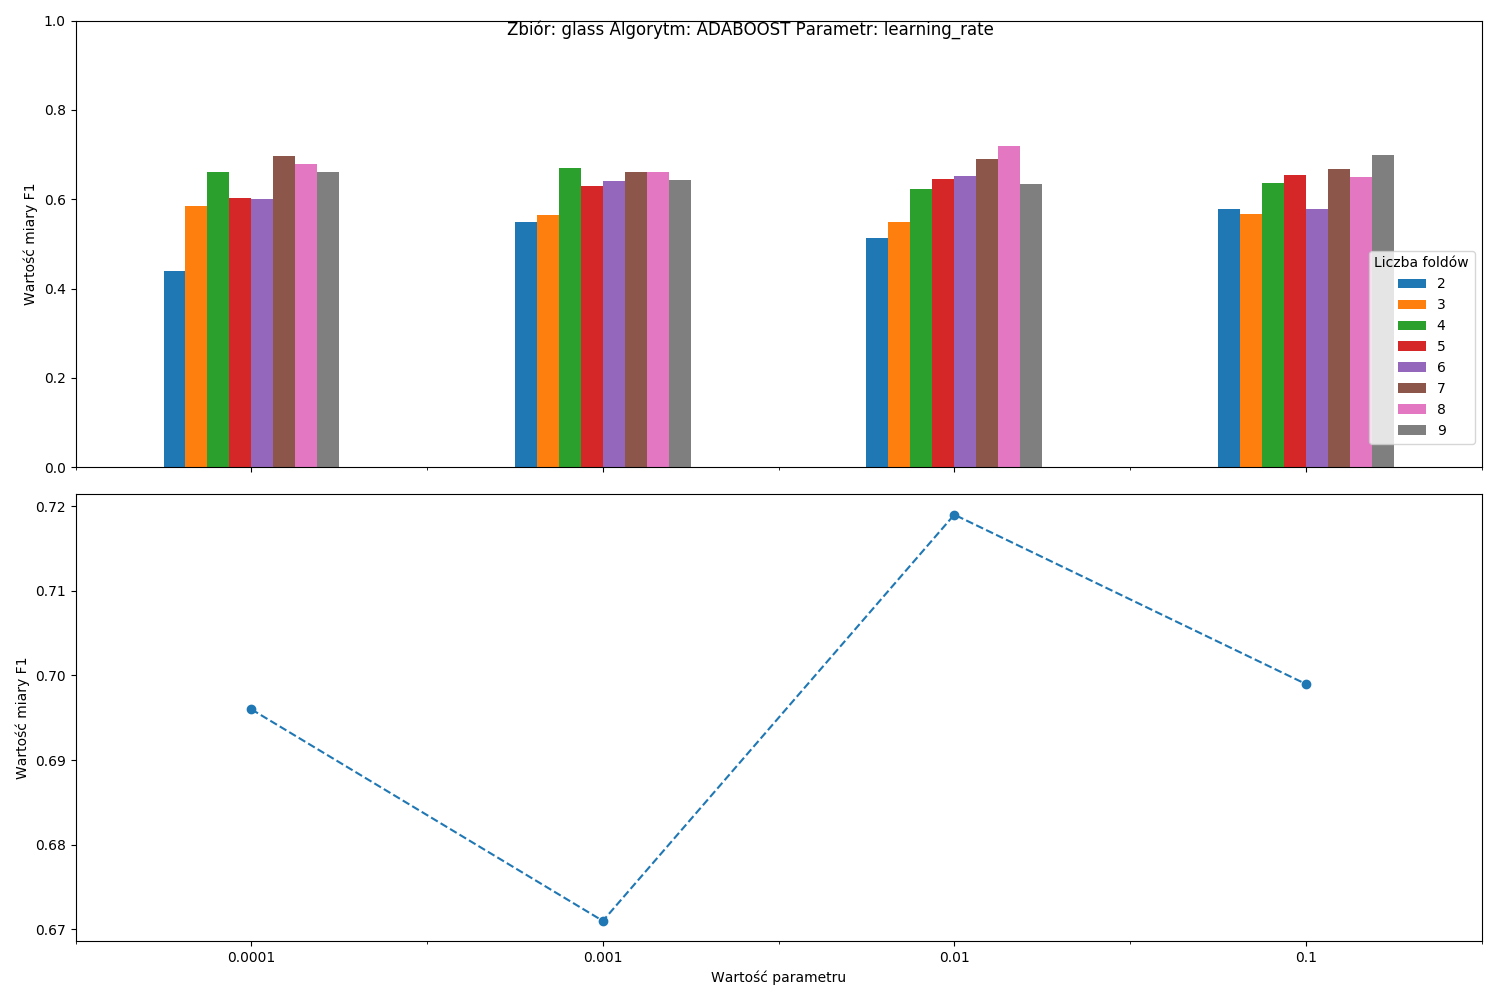
\includegraphics[width=\textwidth]{resources/plots/glass_adaboost_learning_rate.png}
    \caption{Wykres wartości miary F1 dla zbioru "Glass" algorytmu "Adaboost" przy ustalonym parametrze "learning\_rate".}
\end{figure}

\pagebreak
                    
\begin{tabular}{llrrrrrrrr}
\hline
             & \{\} & \multicolumn{8}{l}{Miara F1} \\
             & Liczba foldów &        2 &      3 &      4 &      5 &      6 &      7 &      8 &      9 \\
Parametr & Wartość parametru &          &        &        &        &        &        &        &        \\
\hline
n\_estimators & 10 &    0.606 &  0.598 &  0.647 &  0.669 &  0.655 &  0.682 &  0.717 &  0.666 \\
             & 25 &    0.555 &  0.601 &  0.657 &  0.694 &  0.613 &  0.638 &  0.669 &  0.651 \\
             & 50 &    0.473 &  0.651 &  0.663 &  0.659 &  0.622 &  0.675 &  0.707 &  0.669 \\
             & 75 &    0.526 &  0.580 &  0.617 &  0.641 &  0.665 &  0.641 &  0.639 &  0.612 \\
             & 99 &    0.576 &  0.629 &  0.634 &  0.690 &  0.627 &  0.647 &  0.704 &  0.682 \\
\hline
\end{tabular}

\begin{figure}[H]
    \center
    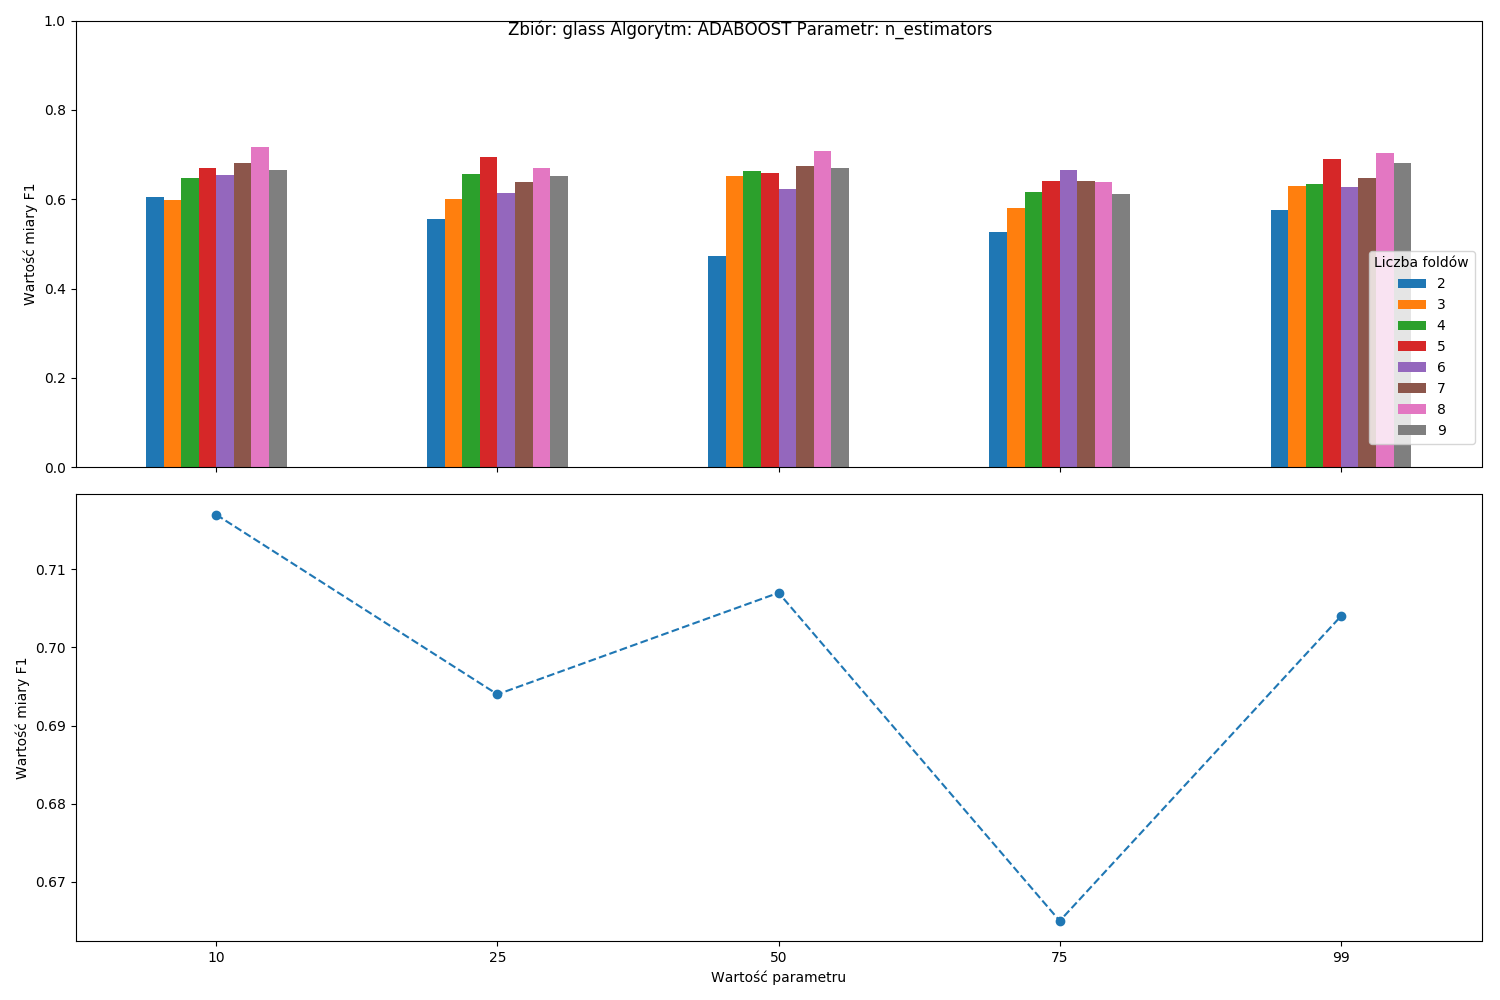
\includegraphics[width=\textwidth]{resources/plots/glass_adaboost_n_estimators.png}
    \caption{Wykres wartości miary F1 dla zbioru "Glass" algorytmu "Adaboost" przy ustalonym parametrze "n\_estimators".}
\end{figure}

\pagebreak
                    
\subsection{Algorytm Bagging}

\begin{tabular}{llrrrrrrrr}
\hline
          & \{\} & \multicolumn{8}{l}{Miara F1} \\
          & Liczba foldów &        2 &      3 &      4 &      5 &      6 &      7 &      8 &      9 \\
Parametr & Wartość parametru &          &        &        &        &        &        &        &        \\
\hline
bootstrap & False &    0.494 &  0.607 &  0.644 &  0.725 &  0.714 &  0.649 &  0.713 &  0.653 \\
          & True &    0.555 &  0.607 &  0.622 &  0.689 &  0.656 &  0.624 &  0.707 &  0.698 \\
\hline
\end{tabular}

\begin{figure}[H]
    \center
    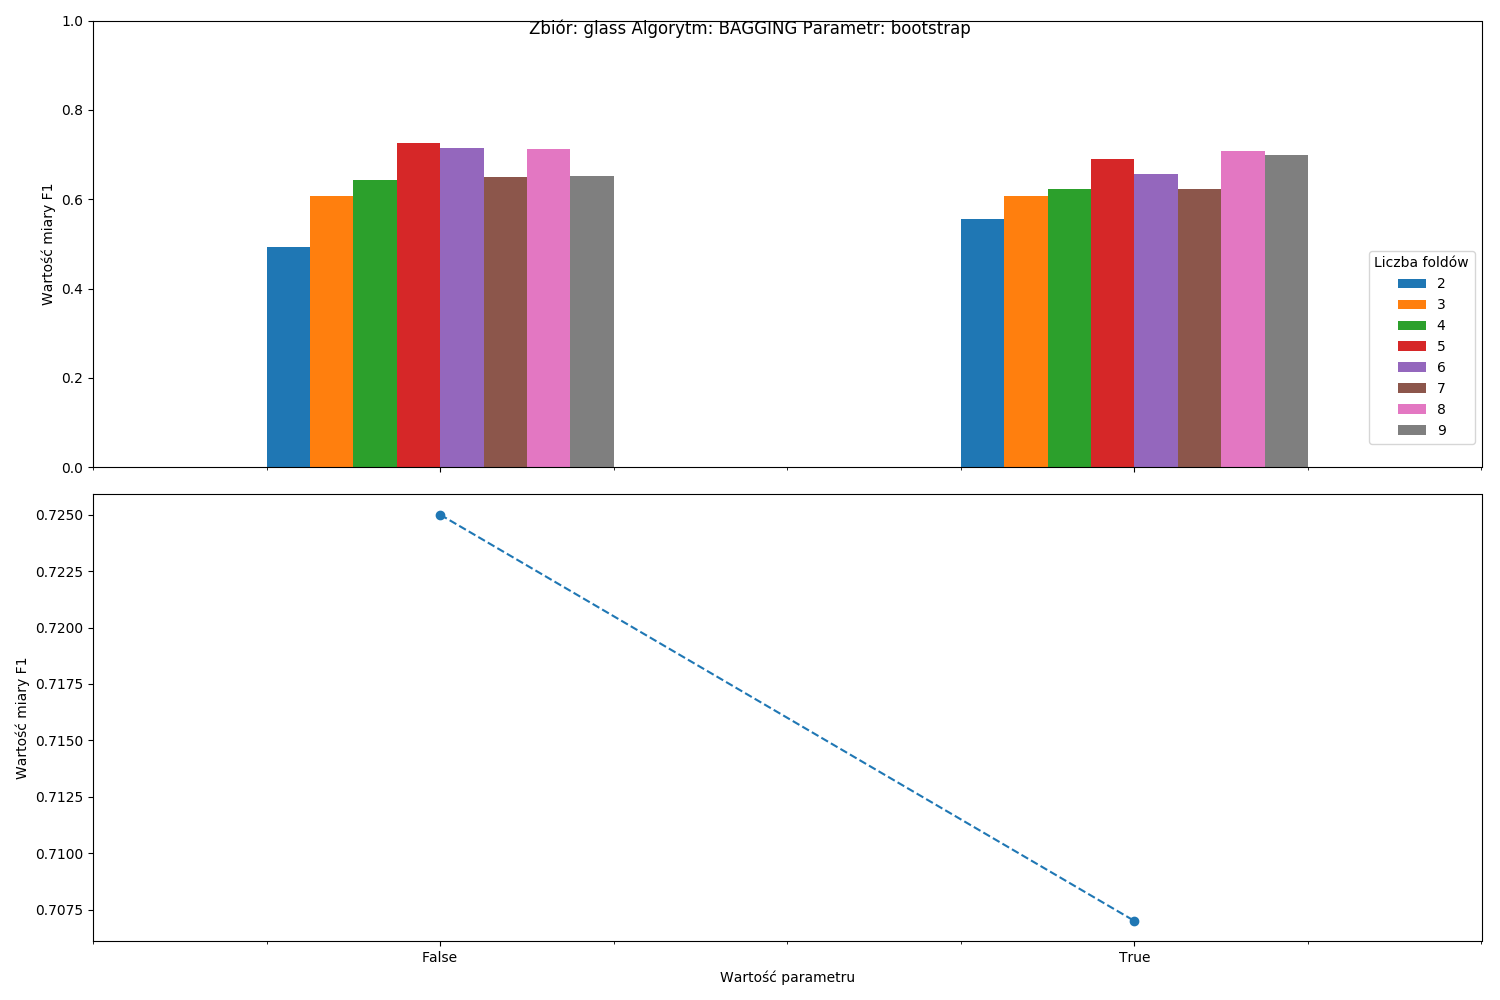
\includegraphics[width=\textwidth]{resources/plots/glass_bagging_bootstrap.png}
    \caption{Wykres wartości miary F1 dla zbioru "Glass" algorytmu "Bagging" przy ustalonym parametrze "bootstrap".}   
\end{figure}

\pagebreak
                    
\begin{tabular}{llrrrrrrrr}
\hline
            & \{\} & \multicolumn{8}{l}{Miara F1} \\
            & Liczba foldów &        2 &      3 &      4 &      5 &      6 &      7 &      8 &      9 \\
Parametr & Wartość parametru &          &        &        &        &        &        &        &        \\
\hline
max\_samples & 0.25 &    0.550 &  0.633 &  0.630 &  0.679 &  0.678 &  0.677 &  0.648 &  0.693 \\
            & 0.5 &    0.520 &  0.610 &  0.602 &  0.710 &  0.642 &  0.652 &  0.707 &  0.664 \\
            & 0.75 &    0.496 &  0.584 &  0.603 &  0.662 &  0.643 &  0.656 &  0.699 &  0.675 \\
            & 1.0 &    0.505 &  0.581 &  0.661 &  0.651 &  0.656 &  0.648 &  0.686 &  0.715 \\
\hline
\end{tabular}

\begin{figure}[H]
    \center
    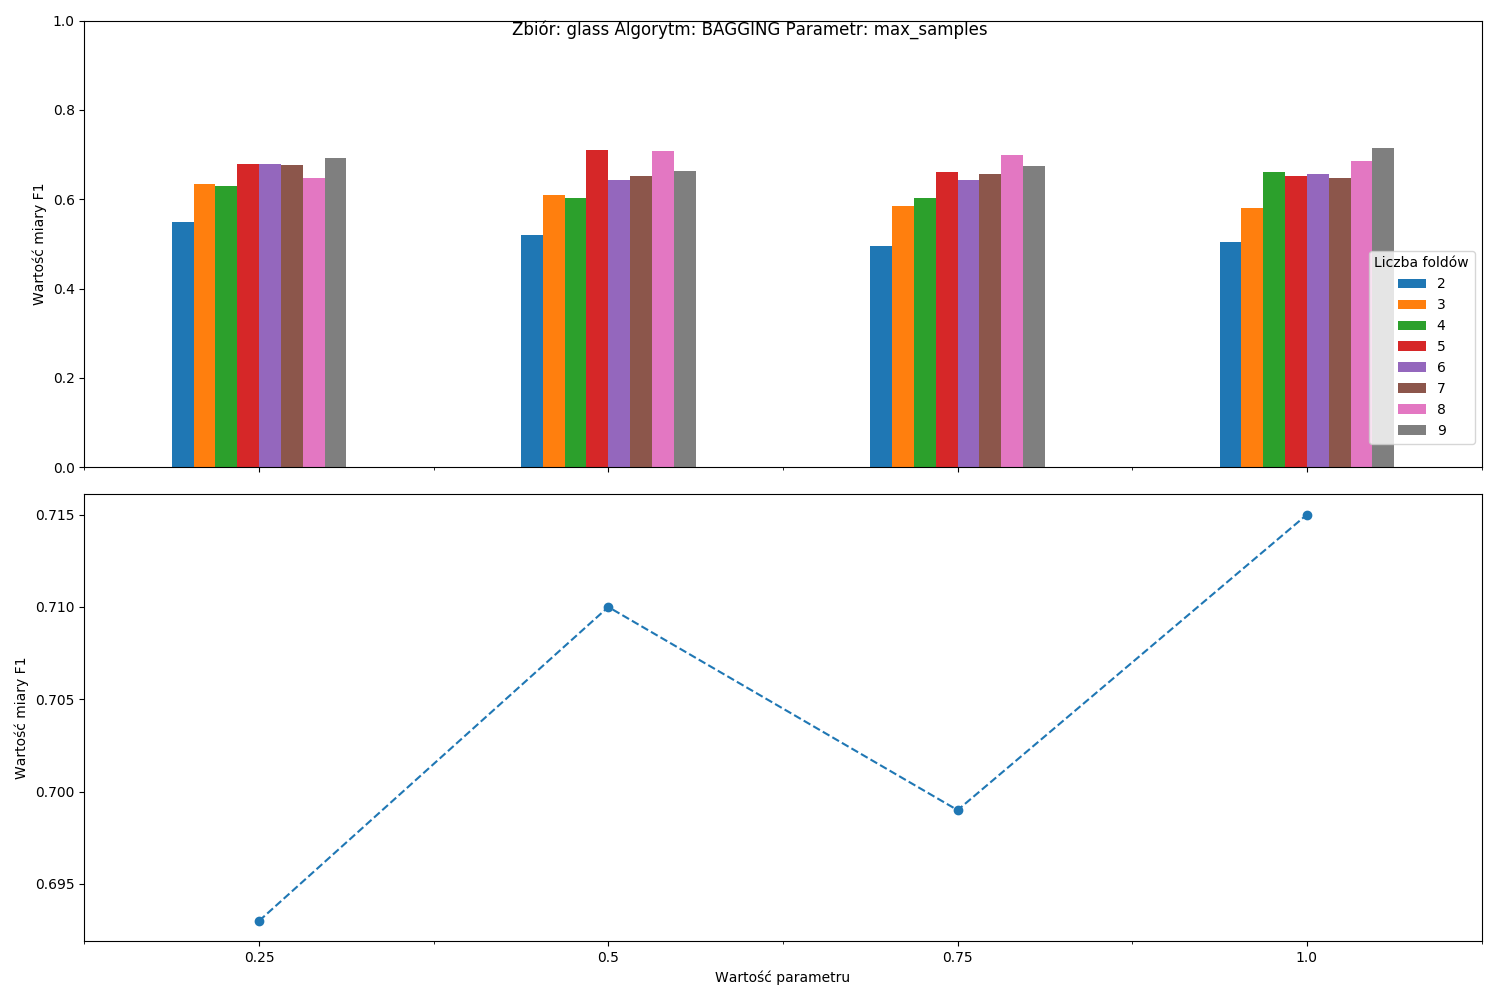
\includegraphics[width=\textwidth]{resources/plots/glass_bagging_max_samples.png}
    \caption{Wykres wartości miary F1 dla zbioru "Glass" algorytmu "Bagging" przy ustalonym parametrze "max\_samples".}
\end{figure}

\pagebreak
                    
\begin{tabular}{llrrrrrrrr}
\hline
             & \{\} & \multicolumn{8}{l}{Miara F1} \\
             & Liczba foldów &        2 &      3 &      4 &      5 &      6 &      7 &      8 &      9 \\
Parametr & Wartość parametru &          &        &        &        &        &        &        &        \\
\hline
n\_estimators & 10 &    0.528 &  0.591 &  0.652 &  0.651 &  0.685 &  0.686 &  0.688 &  0.611 \\
             & 25 &    0.535 &  0.644 &  0.649 &  0.634 &  0.693 &  0.621 &  0.723 &  0.687 \\
             & 50 &    0.507 &  0.606 &  0.659 &  0.667 &  0.610 &  0.643 &  0.700 &  0.627 \\
             & 75 &    0.530 &  0.638 &  0.623 &  0.612 &  0.643 &  0.632 &  0.708 &  0.682 \\
             & 99 &    0.603 &  0.639 &  0.645 &  0.722 &  0.648 &  0.671 &  0.714 &  0.632 \\
\hline
\end{tabular}

\begin{figure}[H]
    \center
    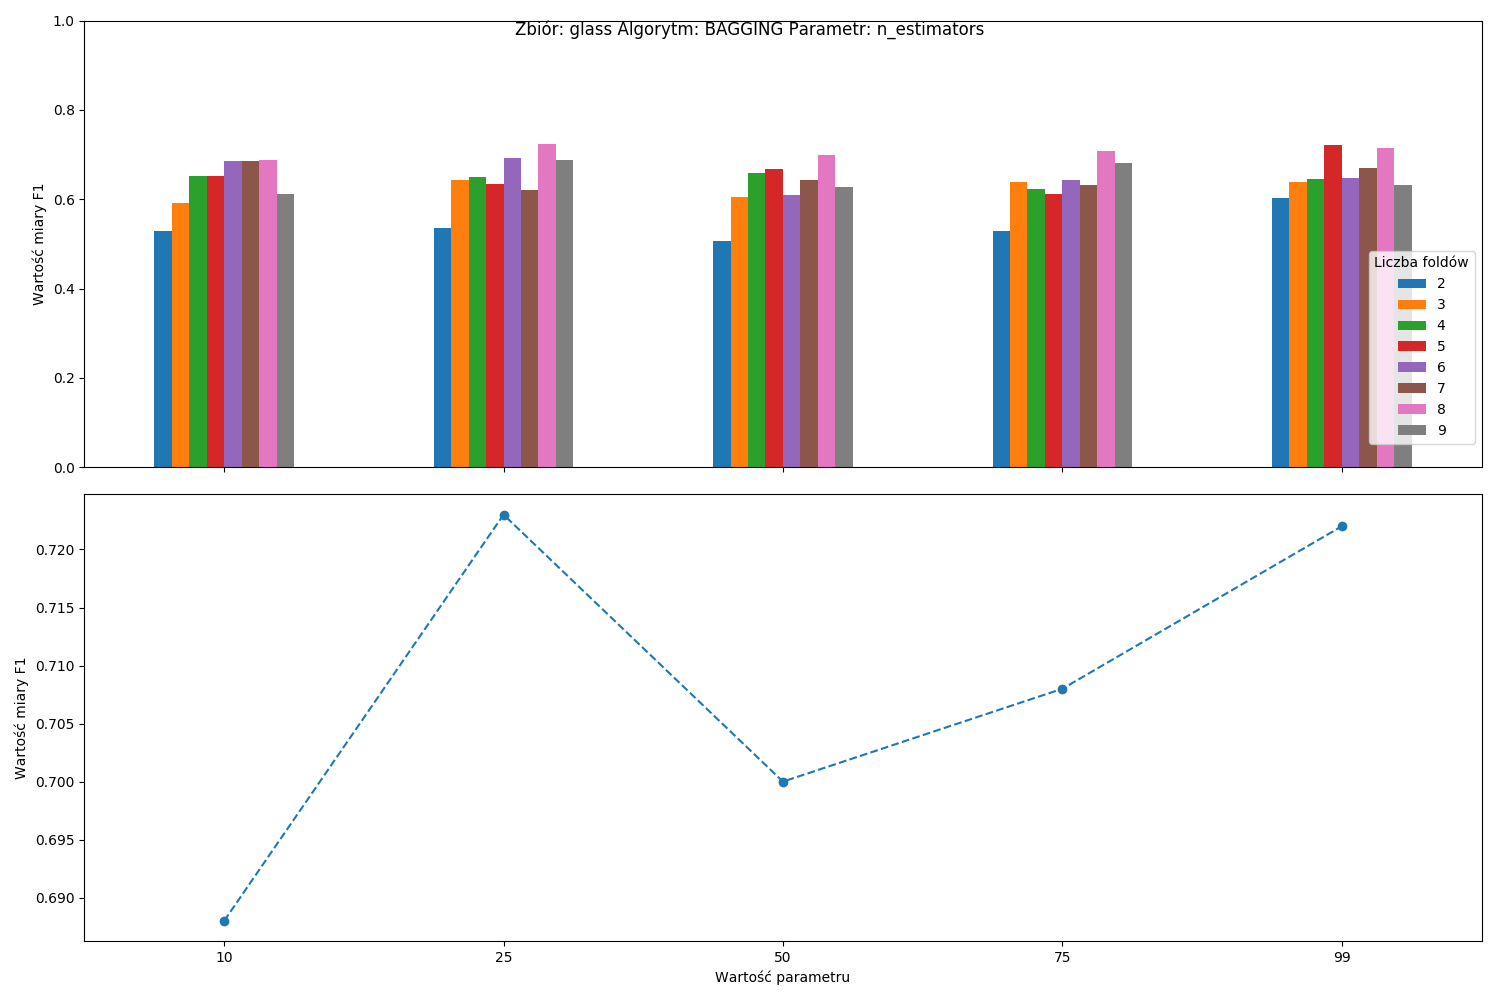
\includegraphics[width=\textwidth]{resources/plots/glass_bagging_n_estimators.png}
    \caption{Wykres wartości miary F1 dla zbioru "Glass" algorytmu "Bagging" przy ustalonym parametrze "n\_estimators".}
\end{figure}

\pagebreak
                    
\subsection{Algorytm Random-forest}

\begin{tabular}{llrrrrrrrr}
\hline
          & \{\} & \multicolumn{8}{l}{Miara F1} \\
          & Liczba foldów &        2 &      3 &      4 &      5 &      6 &      7 &      8 &      9 \\
Parametr & Wartość parametru &          &        &        &        &        &        &        &        \\
\hline
bootstrap & False &    0.467 &  0.635 &  0.708 &  0.663 &  0.658 &  0.625 &  0.710 &  0.682 \\
          & True &    0.523 &  0.607 &  0.587 &  0.651 &  0.633 &  0.608 &  0.684 &  0.627 \\
\hline
\end{tabular}

\begin{figure}[H]
    \center
    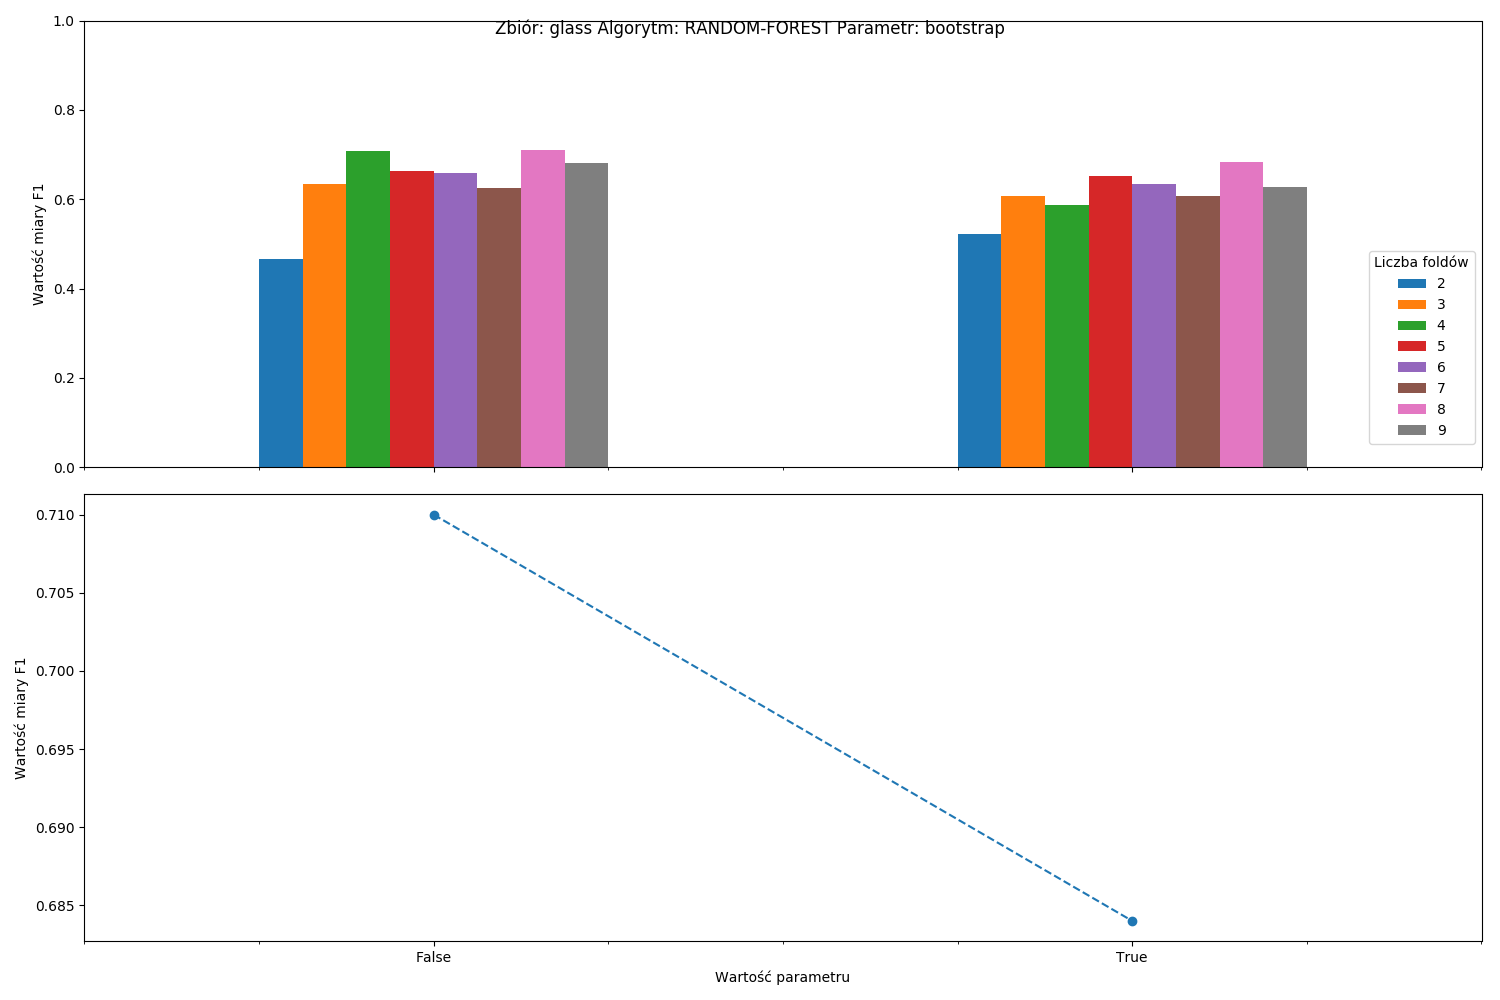
\includegraphics[width=\textwidth]{resources/plots/glass_random-forest_bootstrap.png}
    \caption{Wykres wartości miary F1 dla zbioru "Glass" algorytmu "Random-forest" przy ustalonym parametrze "bootstrap".}   
\end{figure}

\pagebreak
                    
\begin{tabular}{llrrrrrrrr}
\hline
          & \{\} & \multicolumn{8}{l}{Miara F1} \\
          & Liczba foldów &        2 &      3 &      4 &      5 &      6 &      7 &     8 &      9 \\
Parametr & Wartość parametru &          &        &        &        &        &        &       &        \\
\hline
criterion & entropy &    0.563 &  0.654 &  0.668 &  0.676 &  0.669 &  0.666 &  0.75 &  0.637 \\
          & gini &    0.510 &  0.639 &  0.645 &  0.643 &  0.619 &  0.663 &  0.71 &  0.668 \\
\hline
\end{tabular}

\begin{figure}[H]
    \center
    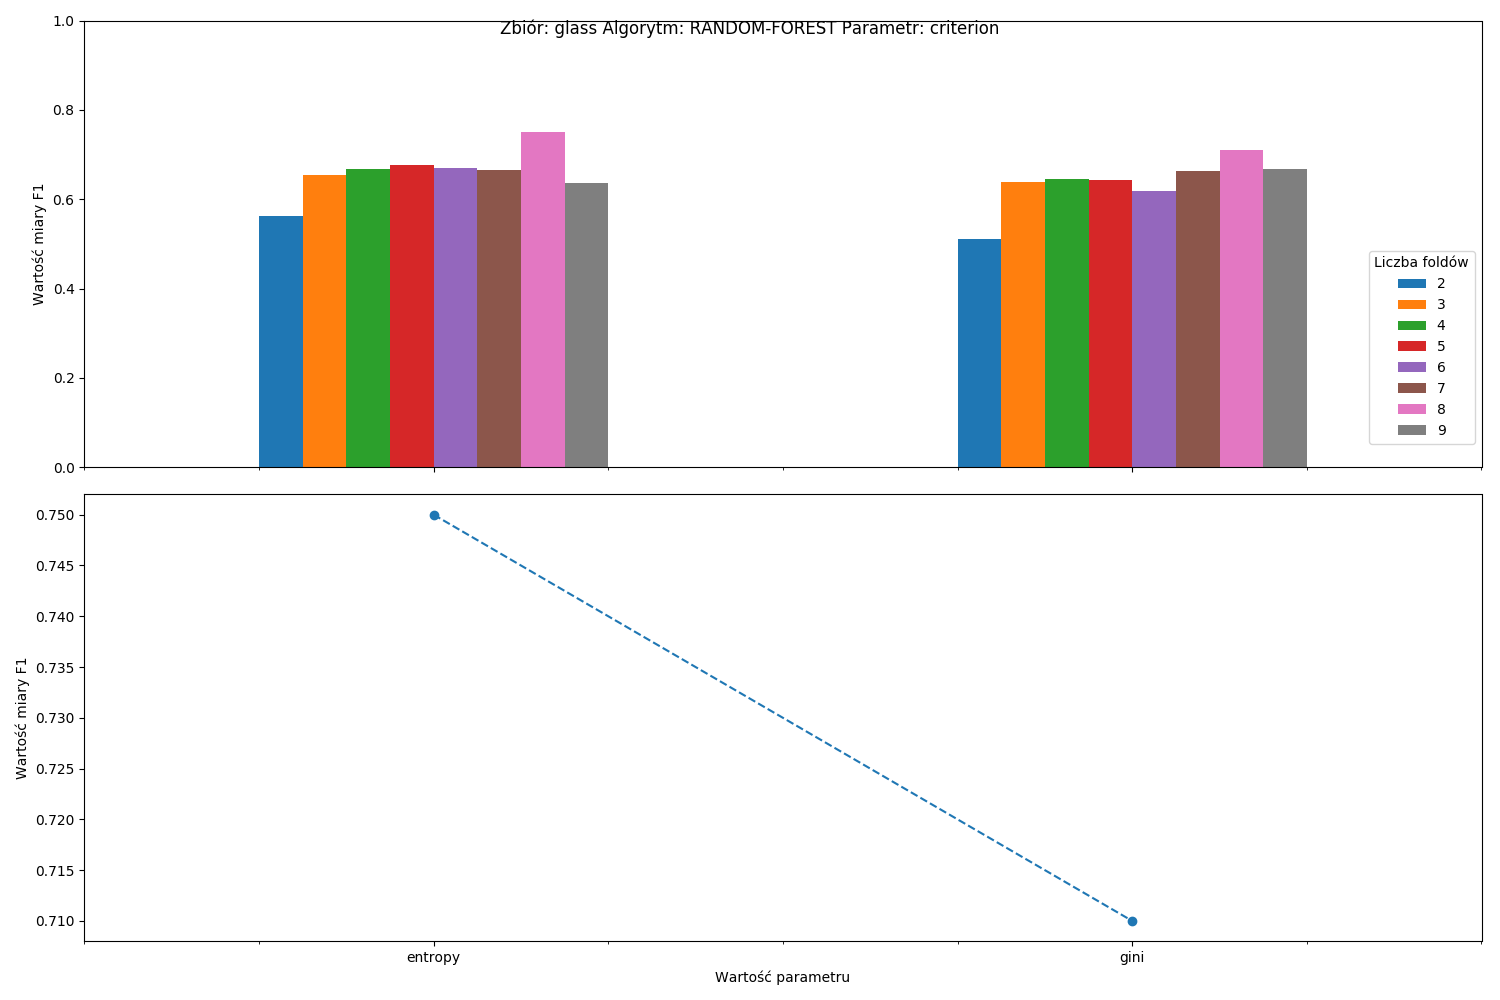
\includegraphics[width=\textwidth]{resources/plots/glass_random-forest_criterion.png}
    \caption{Wykres wartości miary F1 dla zbioru "Glass" algorytmu "Random-forest" przy ustalonym parametrze "criterion".}   
\end{figure}

\pagebreak
                    
\begin{tabular}{llrrrrrrrr}
\hline
             & \{\} & \multicolumn{8}{l}{Miara F1} \\
             & Liczba foldów &        2 &      3 &      4 &      5 &      6 &      7 &      8 &      9 \\
Parametr & Wartość parametru &          &        &        &        &        &        &        &        \\
\hline
n\_estimators & 10 &    0.545 &  0.598 &  0.656 &  0.643 &  0.660 &  0.644 &  0.664 &  0.670 \\
             & 25 &    0.527 &  0.608 &  0.674 &  0.687 &  0.624 &  0.651 &  0.636 &  0.658 \\
             & 50 &    0.511 &  0.599 &  0.612 &  0.610 &  0.683 &  0.625 &  0.657 &  0.637 \\
             & 75 &    0.504 &  0.603 &  0.687 &  0.667 &  0.639 &  0.684 &  0.677 &  0.674 \\
             & 99 &    0.517 &  0.597 &  0.641 &  0.635 &  0.641 &  0.596 &  0.673 &  0.655 \\
\hline
\end{tabular}

\begin{figure}[H]
    \center
    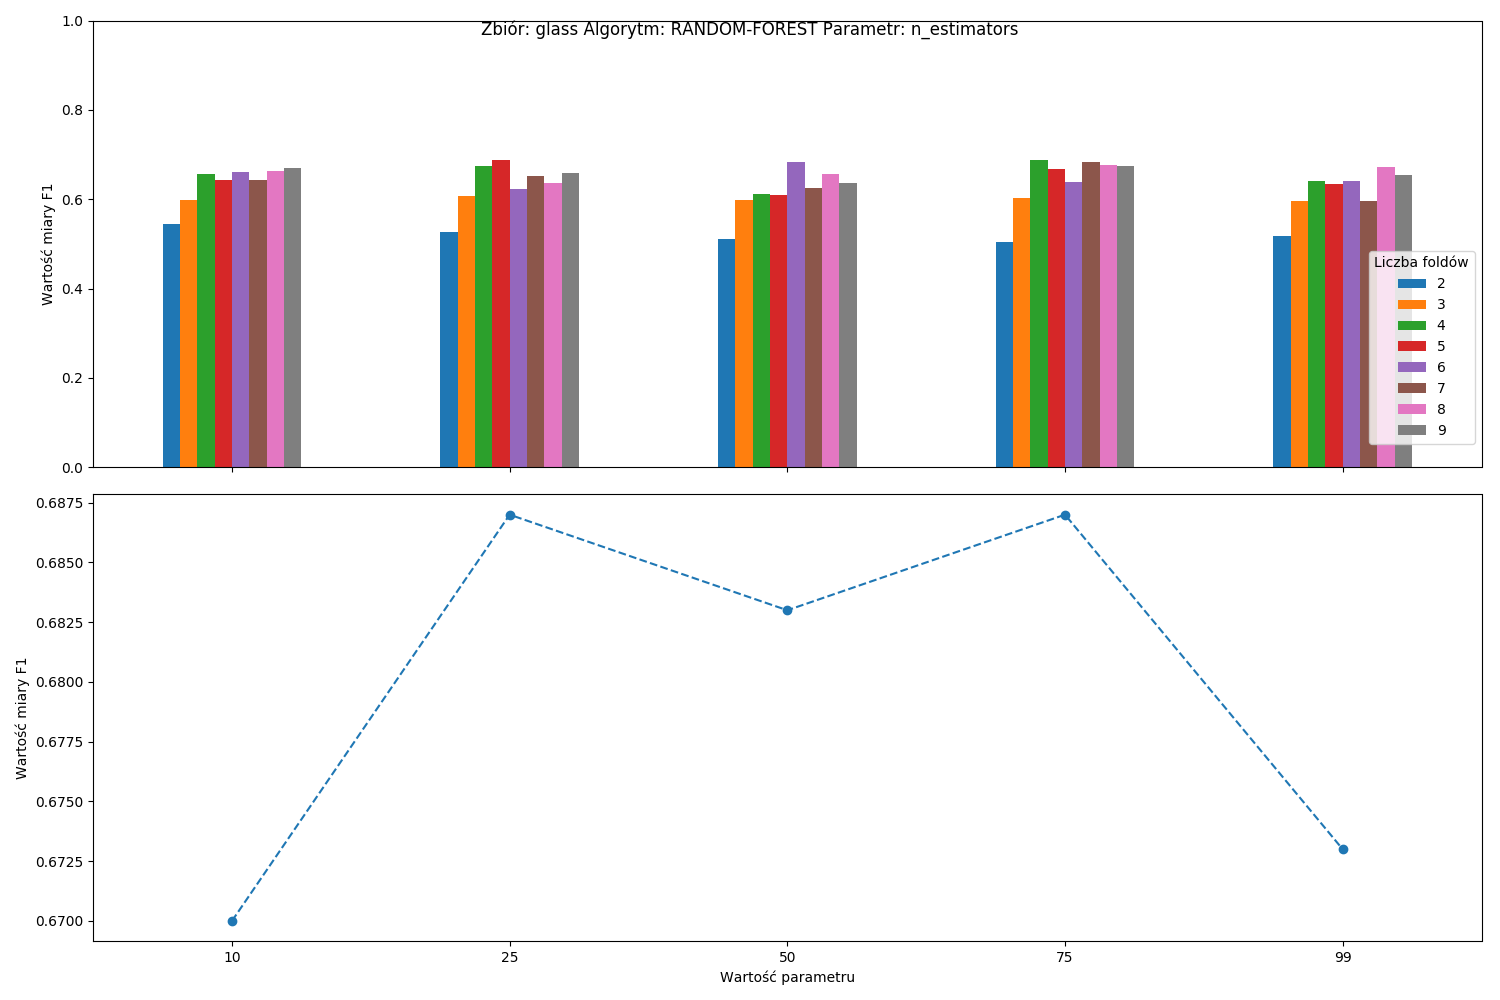
\includegraphics[width=\textwidth]{resources/plots/glass_random-forest_n_estimators.png}
    \caption{Wykres wartości miary F1 dla zbioru "Glass" algorytmu "Random-forest" przy ustalonym parametrze "n\_estimators".}
\end{figure}                    
                    
\pagebreak

\begin{tabular}{llrrrrrrrr}
\hline
             & \{\} & \multicolumn{8}{l}{Miara F1} \\
             & Liczba foldów &        2 &      3 &      4 &      5 &      6 &      7 &      8 &      9 \\
Parametr & Wartość parametru &          &        &        &        &        &        &        &        \\
\hline
max\_features & 0.25 &    0.482 &  0.600 &  0.615 &  0.606 &  0.632 &  0.643 &  0.698 &  0.701 \\
             & 0.5 &    0.520 &  0.597 &  0.619 &  0.658 &  0.622 &  0.644 &  0.701 &  0.644 \\
             & 0.75 &    0.525 &  0.568 &  0.592 &  0.661 &  0.607 &  0.612 &  0.730 &  0.666 \\
             & 1.0 &    0.532 &  0.598 &  0.592 &  0.618 &  0.631 &  0.619 &  0.664 &  0.616 \\
\hline
\end{tabular}

\begin{figure}[H]
    \center
    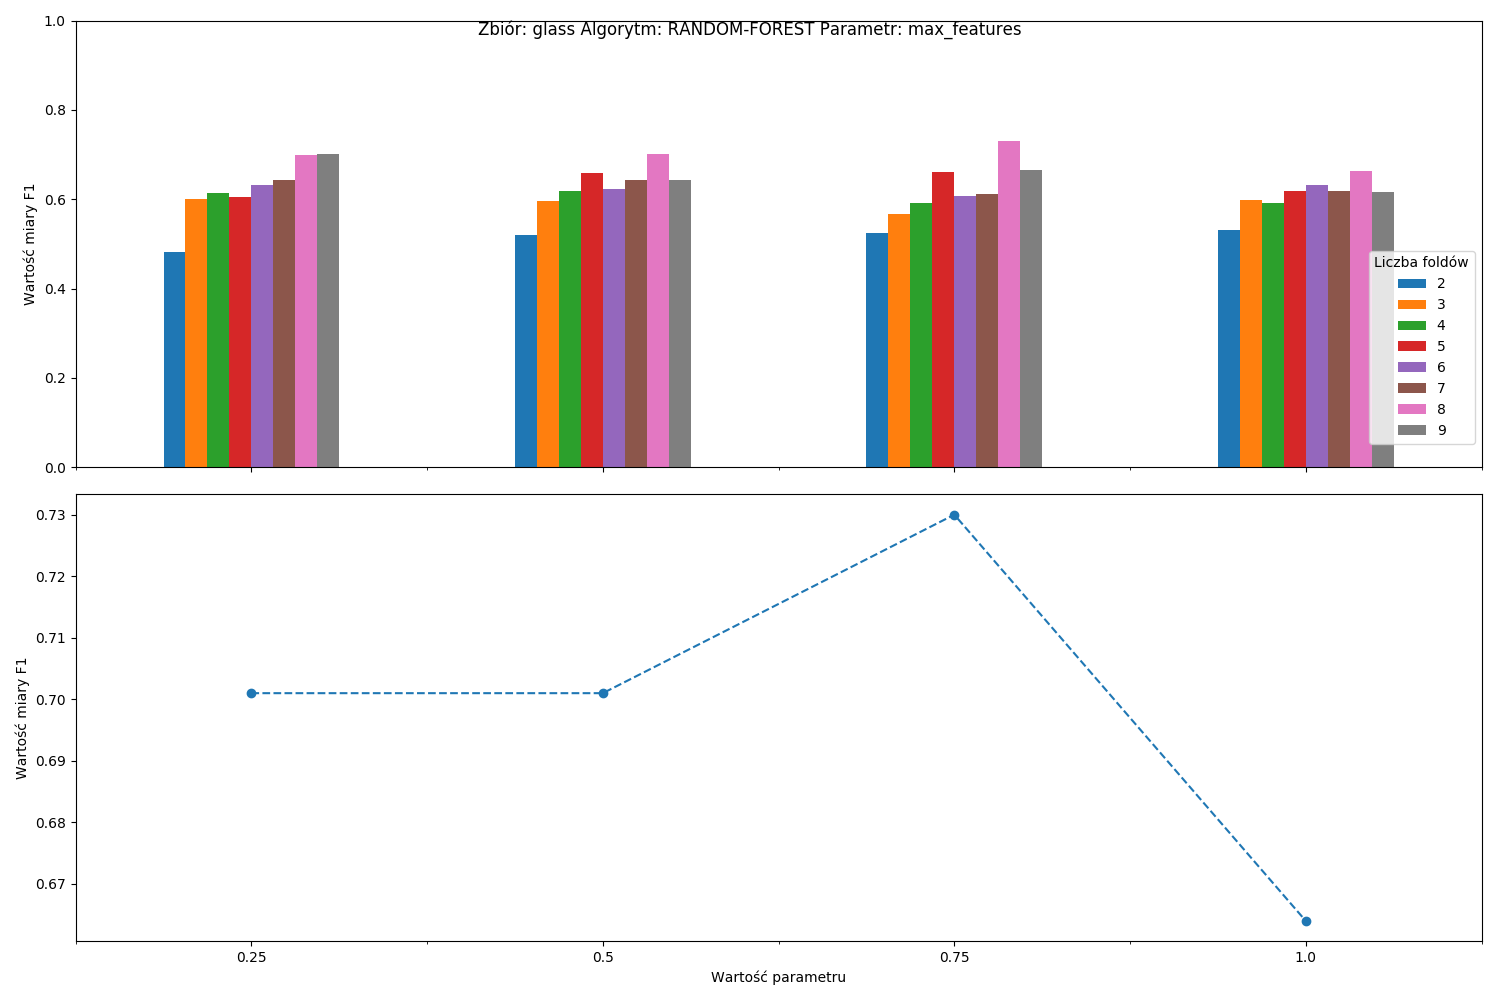
\includegraphics[width=\textwidth]{resources/plots/glass_random-forest_max_features.png}
    \caption{Wykres wartości miary F1 dla zbioru "Glass" algorytmu "Random-forest" przy ustalonym parametrze "max\_features".}
\end{figure}

\pagebreak
